%◆注意事項(本文全体)◆
%
%タイトルに現れる単語・用語をすべて本文中で解説
%略語は,本文中の最初に登場した個所に正式名称を記載 例: IP (Internet Protocol)
%式,方法,システム,技術,アプリケーション,アーキテクチャという用語は,一貫して使用
%不明確な副詞(例: ある程度,かなり,多少,非常に,とても など)は使わず,定量的な表現
%自分が出した結果(結論)は主体的な表現とすべき
%図表の位置はページ中のトップあるいはボトム
%従来方式,関連研究と比較して,自分の研究結果の利点を明示


%◆注意事項(佐藤先生から)◆
%論文に記載する「参考文献」は,著者が論文を執筆する際に参考した文献を意味しているのではありません.
%読者がこの論文を読む際に,論文では十分説明できないので,ここを参考にしてほしいというものです.
%著者の参考ではなく,読者の参考になるものです.
%
%卒論は研究論文であって,解説論文ではありませんので,一般的な技術を丁寧に説明する必要はありません.自分の研究の★内容★に関わる部分のみ,★必要に応じて★一般技術の説明を入れて下さい.自分の研究と関係ない部分は説明する必要はありません.
%
%図は表について,○○に示すだけではなく,その図や表をどのように解釈したらよいのか,内容について説明してください.
%何かの説明を「図に示す」「表に示す」「式に示す」だけではなく,その図,表,式をどう解釈して,どう読み取るのかを文章で記載して下さい.
%
%研究業績は,参考文献と同じように,雑誌名,ページ数,発行年の形式にして下さい.
%
%,「...したい」と記載するのではなく,「◯◯するためには,さらに◯◯が必要である.」みたいな感じがよいと思います.

%図のフォントは,(図全体を小さくして)本文のフォントと同じぐらいの大きさがよいと思います(極端に文字が大きいとカッコ悪い)
 




\documentclass
[a4paper,11pt]{jreport}
\usepackage
{graduatethesis}

\title
{3次元環境認識に基づく死角領域内の\par AR可視化によるドローン操縦性向上}

\author
{竹内 一真}
\department
{情報システムデザイン学科}
\date
{2021年2月12日}
\advisor
{佐藤 健哉 教授}
\entranceyear
{2017}
\registernumber
{63}

\begin{document}
\maketitle
\begin{abstract}

%============================ 概要 ===================================
%研究結果および論文の結論まで含めて書く 
%概要の中では参考文献を引用しないのが一般的
近年,多方面でのドローンを活用した事業が進出しており,屋内での利用も期待されている.中でも小型ドローンは機体が小さいことから,人間が入れないような狭い環境での活躍が期待されている.しかしながら,狭小空間でのドローンの飛行は障害物が多く,遮られた視点からの操縦は困難な場合がある.オンボードカメラ搭載ドローンを用いれば上記の環境でも操縦しやすくなるが,カメラは前方しか映さないため,死角が多くなるという問題が生じる.そこで本研究では,操縦者とドローンの間に障害物が存在し,ドローンを視認できない環境に対してAR(Augmented Reality)を用いる.SLAM(Simultaneous Localization and Mapping)を用いた3次元環境を事前に作成し,障害物の向こう側を可視化し認識する手法を提案した.しかし,操縦者視点での操縦を実現する上で,障害物までの距離が掴めない懸念がある.そこでARを用いることでドローン近傍の障害物を知覚するための方式を提案し,従来の操縦とARを用いた方式を比較した.その結果,ARありの手法では一貫して走行時間,衝突警告回数が減少し,また,障害物を知覚する手法では衝突警告回数が減少し,操縦性の向上を示すことがわかった.

\addkeywords
{AR}{ドローン}{3次元環境}
\vspace{10.5cm}
\renewcommand{\thefootnote}{\fnsymbol{footnote}}

\footnote[0]{本論文に掲載の製品名・会社名等は,一般にそれぞれの会社の商標,または登録商標である.}
\footnote[0]{なお,本文中では\texttrademark ・ \textregistered 等のマークは特に明記していない.}
\end{abstract}


%----------------------------------------------------------------------
%目次作成部分(変更不要)

%ページ番号をギリシャ数字にする
\pagenumbering{roman}
%目次を1ページから始めるために表紙を0ページにする
\setcounter{page}{0}

%目次を作成
\tableofcontents
%改ページ
\newpage
%以降をアラビア数字で振り直します.
\pagenumbering{arabic}
%----------------------------------------------------------------------

%============================ 第1章 ===================================
\chapter{はじめに}
%なぜこの研究をする必要があるのか,一般的な世間の状況と,研究を行う必要性
はじめに,本研究の背景,目的,構成を述べる.

%本論文の構成について述べる.
%----------------------------------------------------------------------

\section{背景}

%◆ 背景と目的
%
% なぜ,この研究をする必要があるのか,一般的な世間の状況と,研究を行う必要性を書く
% 世の中でその問題にどう取り組んでいるかは,一般には「関連研究」のところで説明
% 一般的な背景情報はこの章にまとめる(本文中に一般的背景情報を書くべきではない)
% 論文の技術的な内容や結果を書く必要がない
近年,多方面でのドローンを活用した事業が進出しており,インフラ点検や,人が行けない場所での災害調査など,応用分野を拡大しながら,世界のドローン市場は急速に成長している\cite{AR}.中でも小型ドローンの特徴である機体の大きさを活かして,人間が入れないような狭い空間での活躍の場も増加することが考えられる.しかし,狭小空間でのドローンの飛行は,遮蔽物が多く,遮られた視点からの操縦を必要とするため,操縦は困難な場合がある.
\par
オンボードカメラ搭載ドローンを使用する場合では,操縦者はドローンから送られてくるビデオストリーミング映像を元に操縦が可能となる.このような典型的なドローンの操縦方法では,実際の現実空間を映像として見ながら操縦できるため,安全な距離から狭小空間を探索することができるが,カメラが前方しか写さないという点から一人称視点の操縦では前方以外の死角が多くなり,状況認識が不十分であり\cite{FPV},また,機体の大きさを掴めないという欠点があるため,狭小空間のように狭く,障害物が多いような環境では操縦は困難である.
\par
ドローン中心の一人称視点での操縦に比べて,同じ空間にあるドローンを見ながらの操縦では,ドローン周辺の状況認識を行うことができ,また,ドローンの実際の高さや位置を正確に把握することができる.しかし,操縦者視点での操縦では,障害物までの距離感が掴めない懸念が依然として挙げられる.
大型ドローンでは,自律飛行や障害物回避などの機能が実現されていることが多いが,センサ搭載制限のある小型ドローンでは,障害物回避の支援がないことが多く,衝突の危険性がある.また,障害物回避を搭載していても,狭小空間では障害物回避が行えないことが多い問題点が存在する.

%----------------------------------------------------------------------
\section{目的}
% 本研究では,コネクテッドカーと通信非対応車両が混在する交差点に着目する.優先道路を走行するコネクテッドカーが交差点周辺の車両の存在をセンシングし,非優先道路を走行するコネクテッドカーにV2V通信を用いて情報を共有する手法を提案し,シミュレーションで評価を行うことで,コネクテッドカーが交差点を通過する際の安全性と効率について検討を行うことを目的とする.

本研究では,狭小空間での死角領域内を飛行するドローン操縦に着目する.拡張現実を用いることで,操縦者の死角領域内を可視化し,狭小空間での操縦性の向上を検討する.しかし,操縦者視点での操縦を実現する上で,障害物までの距離感が掴めない懸念を解決するために,ドローン近傍の障害物を検知するAR方式を提案することで,操縦者にとってどのような情報が障害物までの距離感を把握しやすく,小型ドローン操縦の安全性を向上するかについて検討した.

%----------------------------------------------------------------------
\section{本論文の構成}
本論文では,まず第2章で関連研究について述べる.第3章では提案手法の説明を行い,第4章では提案手法の評価・結果について述べる.第5章では結果に基づいて考察を行い,最後に第6章でまとめとする.

%----------------------------------------------------------------------

%============================ 第2章===================================
\chapter{関連研究}
本章では,本研究で扱うARの可能性や,ドローンが障害物を通過する際に影響する事を関連研究で述べ,また,本研究と同様に狭小空間での小型ドローン操縦を行っている関連研究の紹介と問題点を述べる.

\section{Communicating Robot Motion Intent}
Walkerらは,ARが人間とドローンの相互作用をどのように媒介するかを調査することで,ドローンの意図を視覚的に伝えるための一連の明示的・暗示的なデザインを開発し,ユーザ研究で評価を行った\cite{ARinterface}.

その結果,ドローンに対しARを用いたデザインは,ARなしと比べ,課されたタスク効率を大幅に向上させ,ARを用いることでドローンの操縦性を向上させるための直感的で視覚的な合図を提供することが可能であることが示された.

\section{ドローン操縦におけるクロッシング}
山田らは,ドローン操縦する際に,ある幅内を通過するクロッシング操縦での,クロッシングの要素がドローン操縦に与える影響を調査しモデル化を行なった\cite{crossing}.2つの枠の間をドローンで通過させる実験を行い,操縦時間とエラー率を計測した.エラー率とは,ドローンが枠に触れた場合,または枠外に飛行した場合をエラー率としている.

その結果,ドローンのクロッシングにおける操縦時間は,枠の幅と枠間の距離に影響を受け,また,エラー率は,枠の幅の影響を受けることが示された.枠間の距離が大きくなるほど,また枠の幅が小さくなることよりドローン操縦時間が増えることが示され,枠の幅が小さくなるほどエラー率が増加した.また,アンケート結果より参加者は奥行き感覚を掴みにくく,また,ドローンの幅を小さく見積もっていたことによりエラー率が大きくなった要因と考えられた.

本研究では,枠の幅が0.3mの際のエラー率への主効果が見られていたため,ドローンからの衝突の可能性のある距離を0.3mと設定している.

\section{Drone-Augmented Human Vision}
Eratらの研究では,狭小空間でのドローン視点の一人称でのドローン操縦が困難ということで,三人称視点のドローン操縦手法を提案している\cite{AR_drone}.ドローンがSLAM技術で空間マッピングをすることで,空間の仮想現実を構築し,閉鎖環境を見えるようにするというものである.
結果として,ドローンのカメラから配信されるビデオストリーム映像と異なる視点から見たドローンの操縦映像を基に操縦した条件と比較して,HoloLensを通して壁を透過した条件の方が課されたタスクの完了までの操縦時間が半分以下となることが分かった.

しかし,走行の際に障害物に衝突しないように設定してあり,狭小空間での障害物などによる危険性などが提示されていない.また,ビデオストリーム映像と異なる視点から見たドローンの操縦映像を基に操縦した条件ではジョイパッドを使用して操縦してたのに対して,HoloLensを通して壁を透過した条件では指で仮想のドローンを掴んで動かすことで操縦していたため,タスク完了までの操縦時間への有意差が,ARによる空間認識によるものかどうかが示されていない.よって,実際に狭小空間でのドローン操縦性の向上が見られたかどうかを確認するために,衝突の危険性を提示し,また,ドローン操縦法を統一することで,ARによってドローン操縦性向上を示せるかどうかを検討する必要がある.

%============================ 第3章 ===================================
\chapter{死角領域内でのドローン操縦}


%     問題に関して,自分の解決方法を説明
%     問題そのものを簡単に理解できない場合は,問題についても詳解が必要
%     問題をどうやって解決するかを手順を追って解説
%     複数の問題が関連している場合は問題を分離して説明
%     自分の解決方法が従来とどこが違いどう工夫しているかを明記する必要

本章では,提案手法の概要とその動作について述べる.

%----------------------------------------------------------------------

\begin{table}[bt]
	\caption{各方式の特徴}
	\begin{center}
    \includegraphics[scale = 0.5]{img/design_description.eps}
    \label{tab:design}
    \end{center}
\end{table}




\section{概要}
本研究では,操縦者と小型ドローン(以下,ドローン)の間に遮蔽物があり,ドローンを視認できない環境を「死角領域」とする.ドローンは独自の機体の大きさを活かして,狭小空間へ侵入することが期待されているが,そのような狭小空間は,操縦者にとって死角領域になることが想定される.そのような狭小空間での死角領域でドローンを操縦させるためには,現在のドローンの位置や高さを把握し,また,どのような空間を飛行しているか,状況認識が必要である.
\par
そこで,ドローンが飛行している3次元環境を事前に入手し,ARによって3次元環境とドローンを重畳表示することで,死角領域内を飛行するドローン及び死角領域の3次元環境を認識することが可能なAR方式である可視化方式を提案する.
\par
また,ARによって3次元環境とドローンを認識することで,従来のドローン視点のみの一人称視点での操縦と比べ,操縦者視点での操縦が可能となるため,ドローン周辺の状況認識や現在のドローンの位置や高さの把握が容易となるが,ドローンと障害物までの距離感が掴めない等の操縦性の問題がある.
\par
そこで,死角領域内をドローンが飛行している際に,近傍の障害物までの距離が掴めない問題点を解決するために,ドローン周辺の障害物を操縦者が知覚するための2つのARインタフェース方式である距離画像方式,マーカー方式を開発する.本研究では,前述した可視化方式,距離画像方式,マーカー方式の3つの方式と,典型的な操縦法である,ドローンから送られてくるビデオストリーミング映像を元に操縦する手法を一人称視点方式とした4つの方式を比較することで,操縦者にとってどのような情報が,死角領域内での操縦性の向上を示せるか評価した.
各方式の特徴をまとめた物を表\ref{tab:design}に示し,提案手法の動作例を図\ref{tab:overview}に示す.以降の節では一人称視点方式,可視化方式,距離画像方式,マーカー方式の4つの方式の詳細について説明する.


\begin{figure}[p]
	\begin{center}
    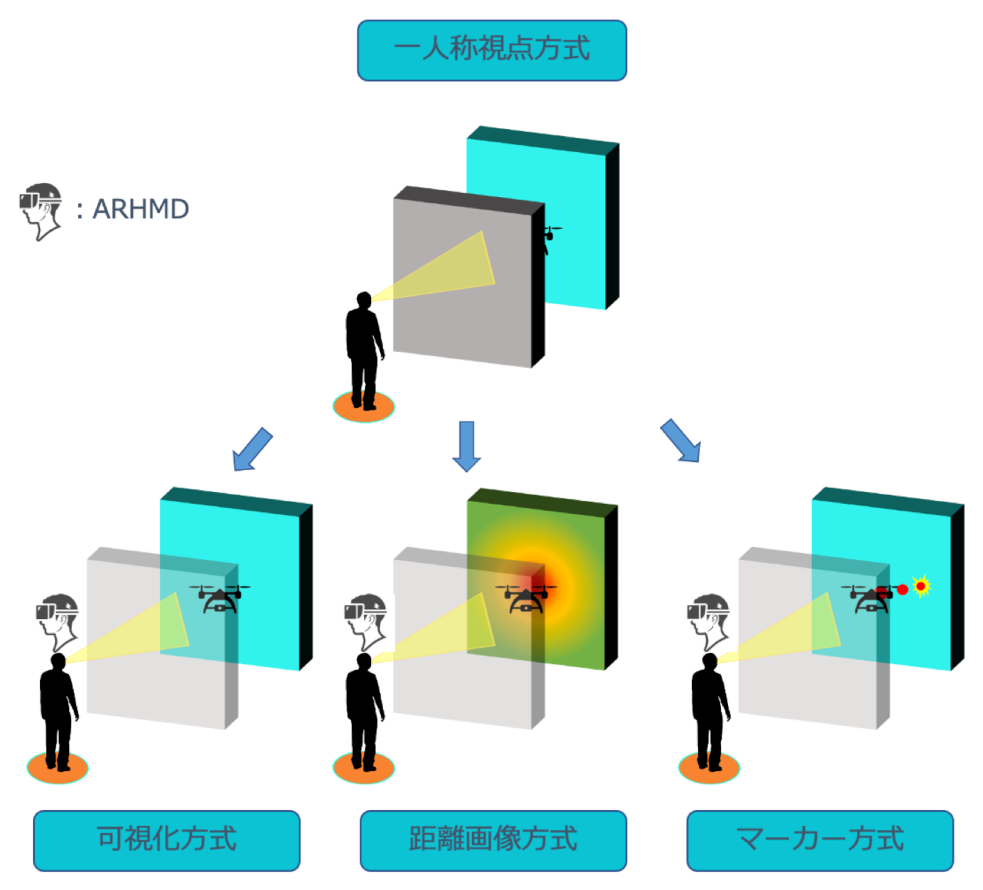
\includegraphics[width=\linewidth]{img/Overview.eps}
    \caption{提案手法の動作例}
    \label{tab:overview}
    \end{center}
\end{figure}

% \section{AR}
% ARは,ユーザが見ている現実のシーンにコンピュータグラフィックスによって描かれた仮想物体を重畳表示することで,ユーザがいる場所に応じた情報を直感的に提示する技術であるcite{}.
% 大部分が現実で仮想物体が部分的に融合し,現実を拡張するという意味で拡張現実感と言われている.

\section{一人称視点方式}
一人称視点方式では,操縦者はドローンから送られてくるビデオストリーミング映像を基に,ドローン中心の一人称視点での操縦を行う.本研究では死角領域内での操縦を前提としているため,操縦者はドローンから送られてくるビデオストリーミング映像のみを頼りに操縦を行う.
\par
実装風景を図\ref{tab:baseline}に示す.
図\ref{tab:baseline}では,左図のドローン視点は,ドローンから送られてきているビデオストリーミング映像を示しており,操縦者はこの映像をもとにドローン操縦を行う.右図の操縦環境では,ドローン操縦を行なっている実際の風景を示しており,操縦者の前には壁があり,操縦者からドローンを視認できない環境となっている.

\begin{figure}[t]
	\begin{center}
    \includegraphics[width=\linewidth]{img/baseline.eps}
    \caption{一人称視点方式}
    \label{tab:baseline}
    \end{center}
\end{figure}

\clearpage

\section{可視化方式}
可視化方式では,ドローンと操縦者の間に遮蔽物が存在すると判断した際,ドローンが飛行している場所を操縦者にとっての死角領域とし,3次元環境地図上の遮蔽物を透過することで,操縦者への死角領域の空間認識を提供する.操縦者は死角領域を飛行するドローンを視認することはできないが,ARによって仮想のドローンと,ドローン周辺の3次元環境を視認することができる.
\par
実装風景を図\ref{tab:visualize}に示す.
図\ref{tab:visualize}では,遮蔽物によって視認できないドローンと,そのドローン周辺の環境をARによって可視化している.障害物を知覚せず,可視化による空間認識の視覚支援のみを行なっている.

\begin{figure}[bt]
	\begin{center}
    \includegraphics[width=\linewidth]{img/visualize.eps}
    \caption{可視化方式}
    \label{tab:visualize}
    \end{center}
\end{figure}

\newpage
\section{距離画像方式}
距離画像方式は,ステレオビジョンを参考にして,ドローンから障害物までの距離に応じて,障害物の色を分けている.距離画像方式は,全体的な環境の理解を提供しており,ドローン周辺の障害物の衝突の危険性を示す.障害物の色分けの際,障害物までの危険な距離を閾値a,未だ猶予はあるが慎重に動くべき距離を閾値bとする.
\par
距離画像方式では常に周りの障害物までの距離を計測し,以下のいずれかの動作をする.

\begin{enumerate}
	\item ドローンからの距離が閾値 a 以内の障害物を赤色に変更
    
    \item ドローンからの距離が閾値a 以降 〜閾値 b 以内の障害物を赤色から黄色に変更
    
    \item ドローンからの距離が閾値 b 以降の障害物を緑色に変更
\end{enumerate}
ここで実装風景を図\ref{tab:stereo}に示す.
距離画像方式は図\ref{tab:stereo}のようにドローン本体ではなく,ドローン周辺の環境を拡張しており,人間の奥行き知覚をサポートしている.赤色になっている障害物の方向にこれ以上進むと衝突の危険性があり,黄色になっている障害物の方向には慎重な操縦を求め,一方で緑色の障害物の方向には進んでも衝突の危険性はないことを示し,操縦者への安心感を与える視覚的支援を行なっている.


\begin{figure}[bt]
	\begin{center}
    \includegraphics[width=\linewidth]{img/stereo.eps}
    \caption{距離画像方式}
    \label{tab:stereo}
    \end{center}
\end{figure}

\clearpage

\section{マーカー方式}
マーカー方式は,ドローンから見て最も近い障害物に対して,目印を付けている.距離画像方式では障害物すべてが色分けされているため,操縦者を混乱させる可能性がある.マーカー方式では,最も危険な障害物のみを知覚させるため,距離画像方式に比べ簡易的なアプローチとなっている.また,マーカー方式でも同じく,障害物の色分けの際,障害物までの危険な距離を閾値a,未だ猶予はあるが慎重に動くべき距離を閾値bとする.
\par
マーカー方式では常に周りの障害物までの距離を計測し,以下のいずれかの動作をする.
\begin{enumerate}
	\item ドローンからの距離が閾値 a 以内の最も近傍の障害物に対して赤色の目印を示す
    
    \item ドローンからの距離が閾値 a以降 〜閾値 b 以内の最も近傍の障害物に対して黄色の目印を示す
\end{enumerate}
実装風景を図\ref{tab:marker}に示す.
マーカー方式は図\ref{tab:marker}のようにドローン自体を拡張しており,ドローンから見てどの方向の障害物が危険か,直感的な理解を支援している.赤色の目印が向けられている障害物はこれ以上進むと衝突の危険性があり,黄色の目印が向けられている障害物は慎重な操縦を求め,操縦者への危機感を与える視覚的支援を行なっている.

\begin{figure}[bt]
	\begin{center}
    \includegraphics[width=\linewidth]{img/marker.eps}
    \caption{マーカー方式}
    \label{tab:marker}
    \end{center}
\end{figure}


%============================ 第4章 ===================================
\chapter{評価}
%    自分の解決方法を問題点に適応してどういう結果が得られたかについて説明
%    従来技術や手法と比較してどこがどうよくなったかを示す
%    どのような環境で比較したかを説明
%    定量的に以前(関連研究)と比べてこうよくなったと説明

本章では,提案手法の実験協力者に関する評価方法や設定と得られた評価結果について述べる.

%----------------------------------------------------------------------

\section{実装環境}
システム構成を図\ref{tab:flow}に示す.
実際に使用したドローンはRyze Tech社製Tello EDU(以下,Tello)であり,操作端末はMacBookProを用いる.Telloはプログラミングによってフライトコントロールを行うことができ,規定のコマンドを送信することで飛行を制御することができる\cite{Tello}.
\par
ARHMDはMicrosoft HoloLens2(以下,HoloLens)\cite{HoloLens}を使用する.
事前にHoloLensのSpatial Mappingにより空間マッピングを行うことで空間のメッシュデータを入手し\cite{spatialmapping},静的な3次元環境地図を作成する.
この3次元環境地図をゲーム・アニメーションエンジンであるUnity\cite{Unity}内の3D仮想空間上に配置し,操縦者とUnity内の3次元環境地図の位置合わせを行うことで,空間認識を提供する.
\par
サーバではTello,HoloLensとUDP通信を行なっており,常時Telloの傾きや,Telloの移動距離をHoloLensに送信することで,3D仮想空間上に存在するドローンの位置合わせを行っている.ここでUDPを使用する理由として,Tello,サーバ,HoloLens間の遅延低減を目的とする.
\par
距離画像方式,マーカー方式では共に障害物までの距離によって,危険度を色で示している.操縦者がドローンを操縦する際の衝突する危険性がある距離を0.3mとし,距離画像方式では,障害物までの距離が0.3mまでを赤色,0.3m\textasciitilde0.6mまでを黄色,0.6m以上を緑色で示す.マーカー方式では障害物までの距離が0.3mまでを赤色のマーカー,0.3m\textasciitilde 0.6mの際に黄色のマーカーを示す.

\begin{figure}[h]
	\begin{center}
    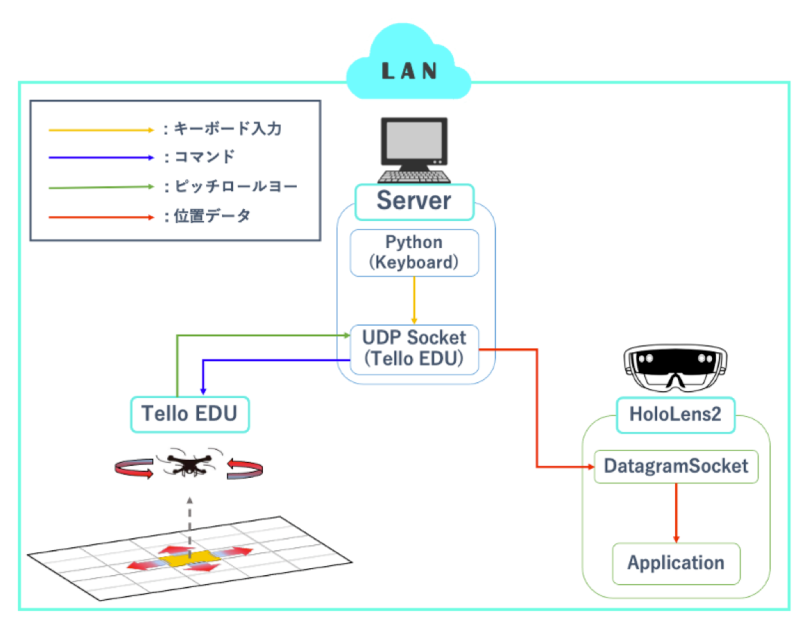
\includegraphics[scale = 0.9]{img/flow.eps}
    \caption{システム構成}
    \label{tab:flow}
    \end{center}
\end{figure}


\section{タスク}
実験環境を図\ref{tab:experiment}に示す.実験環境はスタート地点,障害物,ゴール地点で構成されており,実験参加者はドローンをスタート地点から目的地まで操縦し,目的地で着陸するタスクを行った.その間,上下左右に移動しなければ,衝突の恐れのある障害物を設置した.図\ref{tab:experiment}に赤色で示されている障害物を回避する必要があり,避けなければ通過が困難になるように設定している.実際の狭小空間では,速さより正確な操縦での衝突の減少を求めるため,参加者には早くタスクを終えるのではなく,障害物にぶつかることなく,慎重に通過することを要求した.実験では一人称視点方式,可視化方式,距離画像方式,マーカー方式の計4つの手法で実験を行った.ARを用いた方式では,ドローンの進行方向を分かりやすくするために,ドローンの前方を赤色で示していることを共有する.


%----------------------------------------------------------------------
\begin{figure}[bt]
	\begin{center}
    \includegraphics[scale = 0.8]{img/experiment.eps}
    \caption{実験環境}
    \label{tab:experiment}
    \end{center}
\end{figure}


%----------------------------------------------------------------------

\section{実験}
死角領域内を飛行するドローンの操縦に各方式がどのように影響を与えるかを評価するために10人の実験協力者による実験を行なった.参加者の平均年齢は22歳であり,ドローン操縦経験はなかった.実験は約60分で行い,導入,各提案手法の練習,ARのキャリブレーション,タスク,アンケートの5つのフェーズから構成する.まず,参加者は本研究の概要と,操縦方法の説明を受け,その後,各方式の練習を行う.予備実験で,慣れにより実験後半の操縦時間が速くなったり,ARの経験がないことから戸惑いが生じることで,ドローン操縦への不安が増え,操縦時間が長くなることがわかったため,今回はこの効果を打ち消すために,ドローン操縦を5〜10分ほど練習した後に,各手法で実験環境を1度走行することで,練習量を増やし,慣れによる差異を無くした.次にAR方式では,HoloLensアプリケーションを起動し,現実空間とのキャリブレーションを行い,参加者はHoloLensを装着した.その後,タスクを行い,各方式で目的地点に着陸する度に実験を行なった方式についてアンケートを記入し,全方式を終了したら,どの方式が最も効果的であったかを選択しその理由を記入した.また,なぜ他の方式を選択しなかったのかの理由も記入した.

% \section{評価環境}
% 評価ではドローン技術の熟練度による差を出さないために,Telloの速度,一度に進む距離,旋回角度などは事前に設定している.またサーバとなるPCのスペック,Telloによる送信データパラメータの設定を表\ref{tab:spec}に示す.

%----------------------------------------------------------------------


\begin{table}[bt]
  \begin{center}
  \caption{サーバーのスペックと送信データパラメータ}
    \begin{tabular}{|l|l|} \hline
    \multicolumn{2}{|c|}{サーバーのスペック}\\ \hline
    機器名 & MacBookPro \\ \hline
    OS & macOS 11.0.1 \\ \hline
    CPU & 2.4GHz Intel Core i4\\ \hline 
    メモリ & 8GB\\ \hline 
    使用言語 & Python2.7\\ \hline \hline
    \multicolumn{2}{|c|}{送信データパラメータ}\\ \hline
    前進後退 & 0.3 m\\ \hline
    左右移動 & 0.3 m\\ \hline
    上昇下降 & 0.3 m\\ \hline
    左右旋回 & 20 度\\ \hline
    送信間隔 & 0.3 s\\ \hline
    \end{tabular}
    \label{tab:spec}
  \end{center}
 \end{table}


% \begin{table}[bt]
% 	\caption{サーバーのスペック}
% 	\begin{center}
%     \includegraphics[scale = 1.0]{img/server.eps}
%     \label{tab:server}
%     \end{center}
% \end{table}

% \begin{table}[bt]
% 	\caption{送信データパラメータ設定}
% 	\begin{center}
%     \includegraphics[scale = 1.0]{img/parameter.eps}
%     \label{tab:parameter}
%     \end{center}
% \end{table}


%----------------------------------------------------------------------




%----------------------------------------------------------------------

% \begin{figure}[b]
% 	\caption{アンケート項目}
% 	\begin{center}
%     \includegraphics[width=\linewidth]{img/Likert_1.eps}
%     \label{tab:Likert1}
%     \end{center}
% \end{figure}

% \begin{figure}[b]
% 	\caption{ARのみのアンケート項目}
% 	\begin{center}
%     \includegraphics[width=\linewidth]{img/Likert_2.eps}
%     \label{tab:Likert2}
%     \end{center}
% \end{figure}



%------------------------------------------------------------



\section{評価項目}
評価ではドローン技術の熟練度による差を出さないために,Telloの速度,一度に進む距離,旋回角度などは事前に設定している.またサーバとなるPCのスペック,Telloによる送信データパラメータの設定を表\ref{tab:spec}に示す.
本研究では各手法での,ドローンがスタート地点から目的地に着陸し停止するタスクを完了するまでの操縦時間,障害物への衝突警告回数の2項目の客観的な評価と,参加者へのアンケートの主観的な評価を記録した.障害物の衝突警告回数では,実際に衝突してしまうと危険であるため,操縦者がドローンを進行させようとしている方向に存在する障害物との距離を計測し,距離が0.3 m以内の際に操縦者へ警告がされるようになっている.今回はドローンの進行距離が0.3 mであるため,0.3 mを閾値とした.また参加者へのアンケートでは,主観的な認識と好みを測定するために,7ポイントのリッカート尺度のアンケートを実施した.アンケートでは一人称視点方式とARを利用した3つの各手法を比較できるように実施し,また,AR同士での比較ができるように,ARを用いた方式のみ別途アンケートを実施した.一人称視点方式とARを用いた3つの各方式を比較するアンケートでは,安心な操縦が容易だったか,死角領域内での操縦性が容易だったか,どこの障害物が危険かの理解が容易だったかの3項目を答えた.また,ARを用いた方式のみを比較するためのアンケートでは,状況認識が容易だったか,操縦判断に自信を持つことは容易だったか,距離感を掴むことは容易だったかの3項目を答えた.実験の最後には,参加者にはどの方式が最も操縦性が良かったかを選択し,なぜその方式が良かったのか,また,なぜ他の方式を選択しなかったかの理由を述べた.タスク完了時間には一次元配置分散分析(ANOVA)を用いてデータを分析した.また,ポストホック検定では,Tukey HSD検定を行い,各方式の比較を行なった.衝突警告回数,アンケート結果では,Friedman検定を行い,Bonferroni法の多重比較検定を行い各方式の比較を行なった.



\section{評価結果}
タスクを完了するまでの操縦時間の評価結果を図\ref{tab:time},また,その際の障害物への衝突警告回数の結果を図\ref{tab:collision},アンケートでの各方式での比較の結果と,AR方式のみのアンケート結果を図\ref{tab:safely},\ref{tab:blind},\ref{tab:danger},\ref{tab:AR_situation},\ref{tab:AR_confidence},\ref{tab:AR_distance}に示す.

\clearpage

%------------------------------------------------------------------------
\begin{figure}[bt]
	\begin{center}
    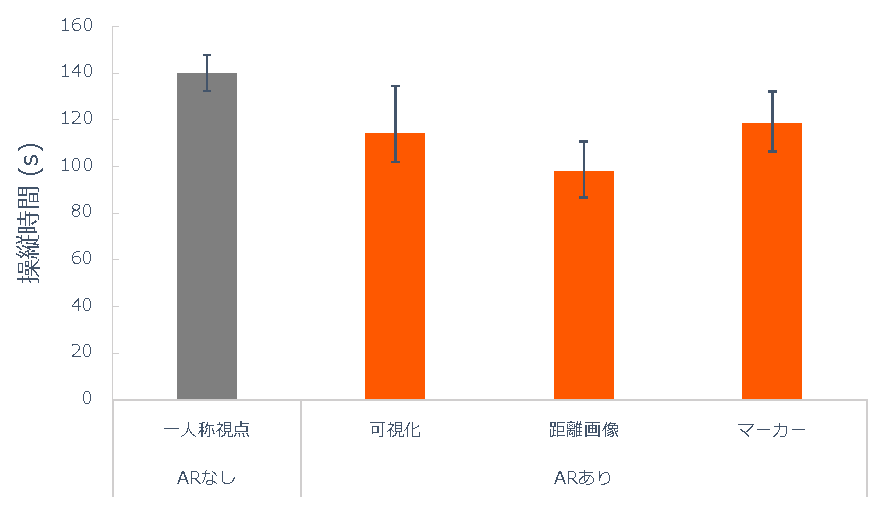
\includegraphics[width=\linewidth]{img/time.eps}
    \caption{操縦時間}
    \label{tab:time}
    \end{center}
\end{figure}

\begin{figure}[bt]
	\begin{center}
    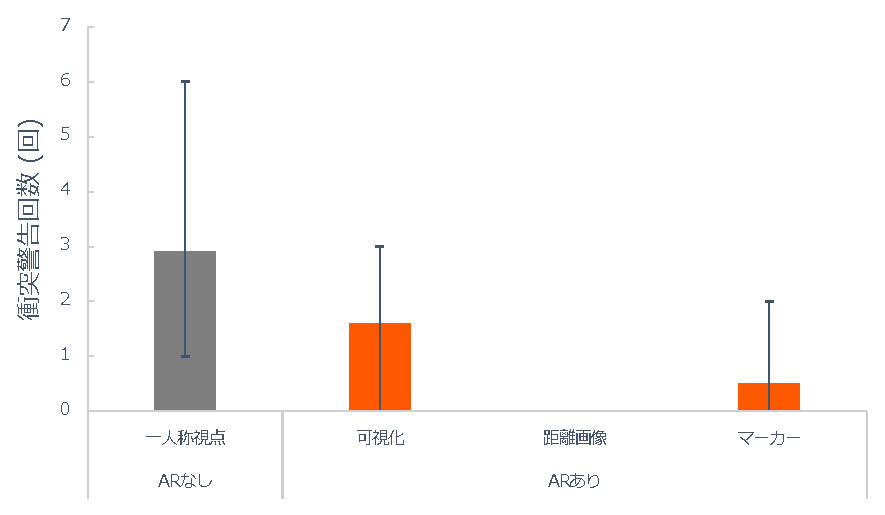
\includegraphics[width=\linewidth]{img/collision.eps}
    \caption{衝突警告回数}
    \label{tab:collision}
    \end{center}
\end{figure}

\begin{figure}[bt]
	\begin{center}
    \includegraphics[scale = 0.8]{img/safely.eps}
    \caption{操縦の安心度}
    \label{tab:safely}
    \end{center}
\end{figure}

\begin{figure}[bt]
	\begin{center}
    \includegraphics[scale = 0.8]{img/blind.eps}
    \caption{死角領域内での操縦性}
    \label{tab:blind}
    \end{center}
\end{figure}

\begin{figure}[bt]
	\begin{center}
    \includegraphics[scale = 0.8]{img/danger.eps}
    \caption{障害物知覚}
    \label{tab:danger}
    \end{center}
\end{figure}

\begin{figure}[bt]
	\begin{center}
    \includegraphics[scale = 0.8]{img/AR_situation.eps}
    \caption{状況認識}
    \label{tab:AR_situation}
    \end{center}
\end{figure}

\begin{figure}[bt]
	\begin{center}
    \includegraphics[scale = 0.8]{img/AR_confidence.eps}
    \caption{操縦判断の自信度}
    \label{tab:AR_confidence}
    \end{center}
\end{figure}

\begin{figure}[bt]
	\begin{center}
    \includegraphics[scale = 0.8]{img/AR_distance.eps}
    \caption{距離感}
    \label{tab:AR_distance}
    \end{center}
\end{figure}

\clearpage
%------------------------------------------------------------------------
\subsection{客観的結果}
図\ref{tab:time}よりタスク完了までの操縦時間ではANOVA(一次元配置分散分析)で4群間に有意差を示し(F(3,36)=48.35,p=1.04e-12)であり,Tukey HSD検定を用いた多重比較では,一人称視点方式とARを用いた方式を比較すると,可視化方式(p<0.001),距離画像方式(p<0.001),マーカー方式(p<0.001)とタスクを完了する時間は有意に減少し,ARを用いた方式同士では,距離画像方式と比較すると,可視化方式(p<0.001),マーカー方式(p<0.001)と有意に時間が減少したことが分かるが,マーカー方式は可視化方式(p = 0.545)と有意にタスク完了時間が減少しないことが分かった.
次に図\ref{tab:collision}より衝突警告回数では,Friedman 検定の結果,有意な差を示したため(p<0.05),Bonferroni法の多重比較(p<0.05)を行ったところ,一人称視点方式とマーカー方式,距離画像方式の間には有意差を示したが,可視化方式との間に有意差は示さなかった(p = 0.163).また,可視化方式とマーカー方式の間には有意差を示しなかったが(p = 0.069),距離画像方式の間には有意差を示した.

\subsection{主観的結果}
一人称視点方式を含むアンケート結果である図\ref{tab:safely},図\ref{tab:blind},図\ref{tab:danger}より,操縦の安心度,死角領域内の操縦性,障害物知覚の3項目全てのFriedman 検定の結果,有意な効果を示した(p<0.05).それぞれの結果に対しBonferroni法の多重比較(p<0.05)を行ったところ,操縦の安心度では,一人称視点方式とマーカー方式,距離画像方式間に有意差を示し,距離画像方式では,可視化方式,マーカー方式共に有意差を示した.死角領域内の操縦性では,一人称視点方式はARを用いた方式全てとの間に有意差を示し,距離画像方式のみ可視化方式との間に有意差を示し,AR方式の中でも最も良い結果になったことを示した.障害物知覚では,一人称視点方式と距離画像方式,マーカー方式の間に有意差を示し,距離画像方式は可視化方式,マーカー方式の間にも有意差を示した.
\par
ARを用いた方式のみを比較したアンケートである図\ref{tab:AR_situation},図\ref{tab:AR_confidence},図\ref{tab:AR_distance}でも,状況認識,操縦判断の自信度,距離感の3項目全てにFriedman 検定の結果,有意差を示した(p<0.05).それぞれの結果に対しBonferroni法の多重比較(p<0.05)を行ったところ,状況認識では,距離画像方式のみ可視化方式とマーカー方式の間に有意差を示した.操縦判断の自信度でも同じく,距離画像方式のみ可視化方式とマーカー方式の間に有意差を示した.距離感では,可視化方式と距離画像方式,マーカー方式の間に有意差を示した.

%============================ 第5章 ===================================
\chapter{考察}
%なるべく考察を章で分ける.
%提案方式に関する「評価」に関して記載する章があるのが一般的かと思いますが,「考察」の章では,従来技術や関連研究と比較して,評価結果がどうであったかを考察して下さい.

本章では,第4章で得られた評価結果における考察について述べる.
%----------------------------------------------------------------------
\section{AR方式の有用性}
ARを用いた方式では一貫して一人称視点方式と比較して有意差を示した.タスク完了までの操縦時間では,ARを用いた方式は一人称視点方式と比較して全て有意に時間が減少しており,作業効率の向上を見込めることが分かった.また,本研究で想定しているようなドローンは最大飛行時間が短いことが問題点とされている中で,距離画像方式は従来の操縦法である一人称視点方式の操縦時間と比較して約30\% 減少しており,大幅な作業効率の増加を望めることが明らかである.衝突警告回数では,一人称視点方式はタスク完了までの平均の操縦時間と,平均の衝突回数より,1分間の間だけで約1.25回も衝突の可能性があり,実際の狭小空間での操縦性の危険性が分かる.ARを用いた方式の中でも可視化方式は一人称視点方式との間に有意な効果を示さなかった.その上可視化方式は一人称視点方式と比較して,アンケート結果から死角領域内の操縦性を向上させることが分かったが,操縦の安心度や,障害物知覚では有意な効果を示さないことより,死角領域の可視化によって操縦者中心の3人称視点で操縦することだけでは,狭小空間での操縦が未だ危険なことを示した.しかし,距離画像方式やマーカー方式のように障害物を知覚するための方式では操縦時間,衝突警告回数共に有意な効果を示しており,ARにって死角領域を可視化するだけでなく,操縦者にとってドローン周辺の障害物に対する視覚的支援を行うことが,ドローン操縦性向上を示すことが明らかとなった.
\section{AR方式の比較の考察}
\subsection{客観的結果}
タスク完了までの操縦時間では,可視化方式とマーカー方式の間で有意差を示さなかった.これは,マーカー方式がドローンから最も近い障害物1つのみに目印をつけることで,その他の障害物までの距離感を掴む感覚が可視化方式と同じであるからと考えられる.可視化方式と比較して操縦時間が長くなっているのは,1箇所のみ危険な場所に目印を付けられていることで,可視化方式よりも慎重に動いてしまうからであると考えられる.参加者へのアンケートから,可視化方式では距離感が掴みにくいことより,思い切って操縦する傾向が見られているため,マーカー方式に比べ慎重に動いていないので,操縦時間がマーカー方式よりも短いことが考えられる:
\par
\vspace{5mm}
{\rm P[8]}:"一方向でしか近づいている点が分からなかったため,操縦の際に躊躇ってしまうことがあった"
\par
{\rm P[1]}:"可視化方式では,距離感が掴みにくいため,思い切って進むと障害物に当たりそうな場面が
\par 何度かあった"
\par
\vspace{5mm}
また,衝突警告回数では,一人称視点方式と可視化方式との間では有意差を示さず,これはARによって空間認識を提供するだけではドローン周辺の障害物との距離感が掴めないことがアンケートによる感想などから考えられる.距離画像方式,マーカー方式は一人称視点方式との間に有意差を示し,距離感の問題点を解消していると考えられる.また,距離画像方式とマーカー方式の間では有意差を示さなかった.しかし,実際にドローン操縦を行う際にドローンの衝突は0に収めなければならないことを考えると,距離画像方式での衝突警告回数が0回というのは大いに有意な結果である.

\subsection{主観的結果}
アンケート結果では,可視化方式とマーカー方式の間では一貫してあまり有意差を示さなかった.これは,タスク完了時間の際にも述べた,マーカー方式の,ドローンから最も近い障害物のみに目印を示すという特徴によるものであると考えられる.ドローン周辺に衝突の可能性のある障害物が2つ以上ある際に,操縦者が手に入れたい障害物までの距離感を示さない場合があったため,可視化方式とあまり差が出なかったことが分かる:
\par
\vspace{5mm}
{\rm P[5]}:"マーカー方式では,気になる障害物に対してマーカーが出ていない場合がある"
\vspace{5mm}
\par
\section{全体の考察}
実験の最後にどの方式が最も効果的であったかを選択してもらった結果,9名が距離画像方式を選択し,1名がマーカー方式を選択した.距離画像方式を選択した理由として,距離を色で示していることによって距離感を掴みやすかった点や,見える景色全体に色がついているため,どの範囲で動かせば良いかが分かりやすかった点などが挙げられた.逆に他の方式を選択しなかった理由として,ベースライン方式では,上下の障害物までの距離感が掴づらかった点や,周囲の確認に不安があった点などが挙げられ,可視化方式では,全体像は掴めたが状況認識が難しかった点や,距離感に自信を持てない点などが挙げられ,マーカー方式では,一方向でしか距離感が分からなかった点や,距離画像の方が全体像が理解できた点などが挙げられた.一方でマーカー方式を選択した参加者は,一番近い場所を示してくれる安心感がある点からマーカー方式を選択し,距離画像方式では周囲が赤色になった際に困惑した点や,見えている情報が簡潔でない点などから,距離画像方式を選択しなかった.
以上より,狭小空間での操縦では障害物知覚が必要であり,操縦者は,ドローン周辺の障害物全ての距離感の表示を好むことより,最も危ない位置を示すような直感的な情報ではなく,常に周囲の危険性を示す全体的な情報を把握することが重要であることが分かった.距離画像方式では他の方式に比べ操縦時間の大幅な減少,衝突回数の大幅な減少,死角領域内での状況認識の向上を提供できることより,死角領域内での狭小空間の環境下においての操縦性の向上に有効であるといえる.



%----------------------------------------------------------------------
% \section{提案手法の問題点}
% 交通量の多い場合は,優先道路に車両が入り込む隙間がなくなるため,提案手法では限界がある.また,頻繁に情報の送受信を行うことから通信トラフィックの増大で不具合が起きる可能性も考慮すると,都市部の大規模な交差点などでは提案手法は不向きである.この場合には,信号機による調停を行うか,非優先道路のコネクテッドカーが通信によって優先道路のコネクテッドカーに進入依頼を出すような手法の検討が必要となる.


% また,提案手法は車載のレーダセンサによって交差点が見通せることを前提としているため,センサ視野の限界を超えるような曲率の大きなカーブが交差点の前後に存在する場合は提案手法を用いることができない.



%============================ 第7章 ===================================
\chapter{まとめ}
%    * 800 字から1000字ぐらいでまとめてください.(卒論は気にしなくて良い)
%    * 背景,解決すべき問題点,提案内容,結果,考察,研究の意義などを含めて記載してください.
%    * 結果については,過去形(・・・実施した.・・・評価した.・・・確認した.など)で記載してください.
%    背景,解決すべき問題点,提案内容,結果,考察,研究の意義がすべて含まれているか
%検討項目や今後の課題は「考察」に記載し,「まとめ」に記載しないこと)
小型ドローンでの遮られた視点からの狭小空間での操縦は死角の多さや,ドローンと障害物までの距離感が測れないことが懸念されている.本研究では操縦者の死角領域内に存在するドローンと周辺を可視化し,ドローン周辺の障害物を知覚するためのAR方式を提案し,実験を行うことで,遮られた視点からの狭小空間でのドローン操縦性を評価した.結果として,ARを利用した手法では実験環境での操縦時間が短く,衝突回数も少なかったことから,狭小空間での死角領域内のドローン操縦性の向上を示せた.
また,障害物を知覚するためのAR方式では,ドローン周辺の障害物に危険度を色で振り分けている手法が,操縦者への安心を与え,操縦性を向上させたことが確認でき,操縦者は死角領域内でのドローン操縦の際に,なるべく多くの明確な情報を欲し,安心感を求めに行くことが分かった.このことから,ARを用いることで,タスク効率,ドローン操縦性を向上させることができ,また,安心に安全に操縦させるための視覚的支援を行える可能性を示せた.





%============================ 謝辞 ===================================
\chapter*{謝辞}
\thispagestyle{empty}
本研究に際して,多大なご指導とご支援を頂きました同志社大学理工学部情報システムデザイン学科ネットワーク情報システム研究室の佐藤健哉教授に心よりお礼申し上げます.
また,研究内容について親身にアドバイスをくださった上原夏紀先輩,林聡一郎先輩をはじめとした先輩方,研究室の皆様に感謝致します.
最後に,学校生活や研究活動を支えてくれた家族と友人への感謝を持って謝辞を締めさせていただきます.


%============================ 参考文献 ==============================
%    * 勉強した書籍を列挙するものではない    .
%    * 本文中に引用した技術などを記載
%    * 参考文献の番号は,必ず本文中の引用場所を示す
%著者,タイトル,出典,年号の形式は例の通りに正確に記載
%(例:周 劼, 綾木 良太, 島田 秀樹, 佐藤 健哉, クラウドサービスにおける分散コンポーネントフレームワークの提案, 情報処理学会論文誌, Vol.52, No.2, pp.415-423, 2011.)
%参考文献は,URLなどの参照以外に,★論文★が5以上
%単に勉強のために参考にした書籍は列挙する必要なし.


\begin{thebibliography}{99}
\thispagestyle{empty}
\bibitem{AR}
野波 健蔵, ドローン技術の現状と課題およびビジネス最前線, 情報管理, Vol.59, No.11, pp.755-763, 2017.

\bibitem{FPV}
S. A. Green, J. G. Chase, X. Chen and M. Billinghurst, Evaluating the Augmented Reality Human-Robot Collaboration System, 2008 15th International Conference on Mechatronics and Machine Vision in Practice, Auckland, pp. 521-526, 2008.

\bibitem{ARinterface}
M. Walker, H. Hedayati, J. Lee and D. Szafir, Communicating Robot Motion Intent with Augmented Reality, HRI '18: Proceedings of the 2018 ACM/IEEE International Conference on Human-Robot Interaction, pp.316-324, 2018.

\bibitem{crossing}
山田開斗, 薄羽大樹, 宮下芳明, ドローン操縦におけるクロッシング評価, 研究報告ヒューマンコンピュータインタラクション(HCI), Issue.2, No.2, pp.1-6, 2019.

\bibitem{AR_drone}
O. Erat, W. A. Isop, D. Kalkofen and D. Schmalstieg, Drone-Augmented Human Vision: Exocentric Control for Drones Exploring Hidden Areas, in IEEE Transactions on Visualization and Computer Graphics, vol.24, no.4, pp.1437-1446, 2018.


\bibitem{Tello}
Ryze Tech,Tello ダウンロード, https://www.ryzerobotics.com/jp/tello-edu/downloads (参照 : 2020/7)

\bibitem{HoloLens}
HoloLens 2 - 概要、機能、仕様 | Microsoft HoloLens, https://www.microsoft.com/ja-jp/hololens/hardware (参照 : 2020/9)

\bibitem{spatialmapping}
空間マッピング - Mixed Reality | Microsoft Docs, https://docs.microsoft.com/ja-jp/windows/mixed-reality/design/spatial-mapping (参照 : 2020/10)

\bibitem{Unity}
Unity Technologies, https://unity.com/ja (参照 : 2020/5)

\end{thebibliography}


%============================ 研究業績===================================
\renewcommand{\bibname}{研究業績}
\begin{thebibliography}{99}
\thispagestyle{empty}


\item[1) ]竹内一真,上原夏紀,林聡一郎,佐藤健哉,"3次元環境認識に基づく死角領域内のAR可視化によるドローン操縦性向上",情報処理学会 第83回全国大会(発表予定)

\end{thebibliography}

\end{document}
